\documentclass[article.tex]{subfiles}
\begin{document}

\section{Periodic conformal parametrization}
\label{sec:conformal-parameterization}

\begin{figure}[tb]
  \centering
  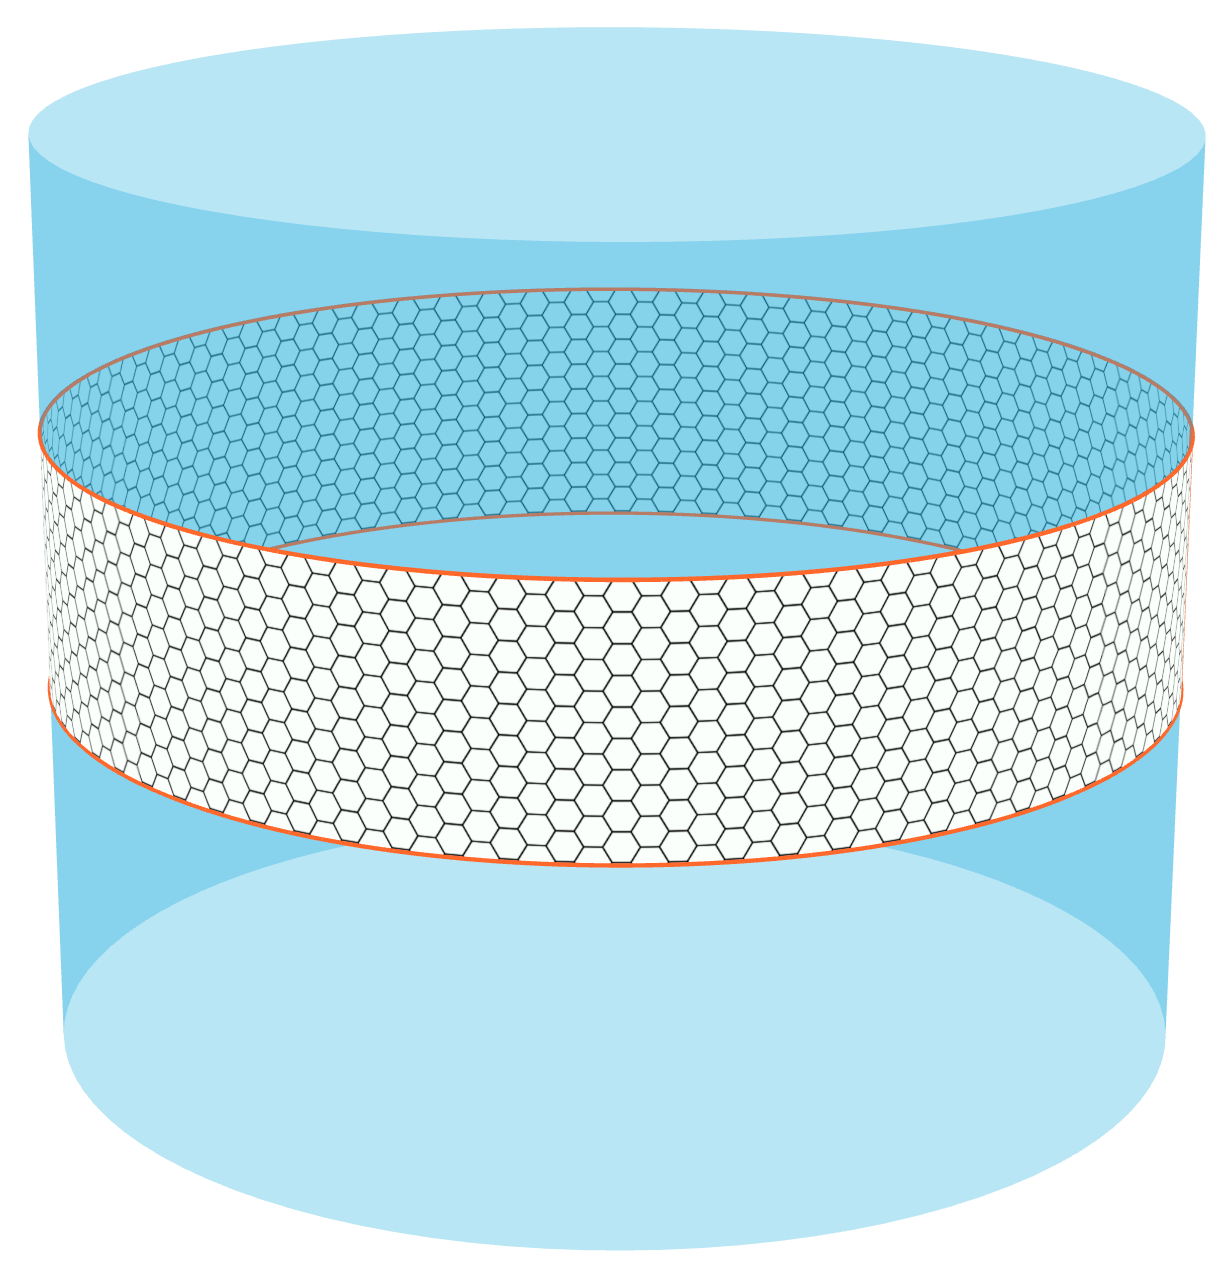
\includegraphics[width=.28\linewidth]{images/conemap_aligned.png}
  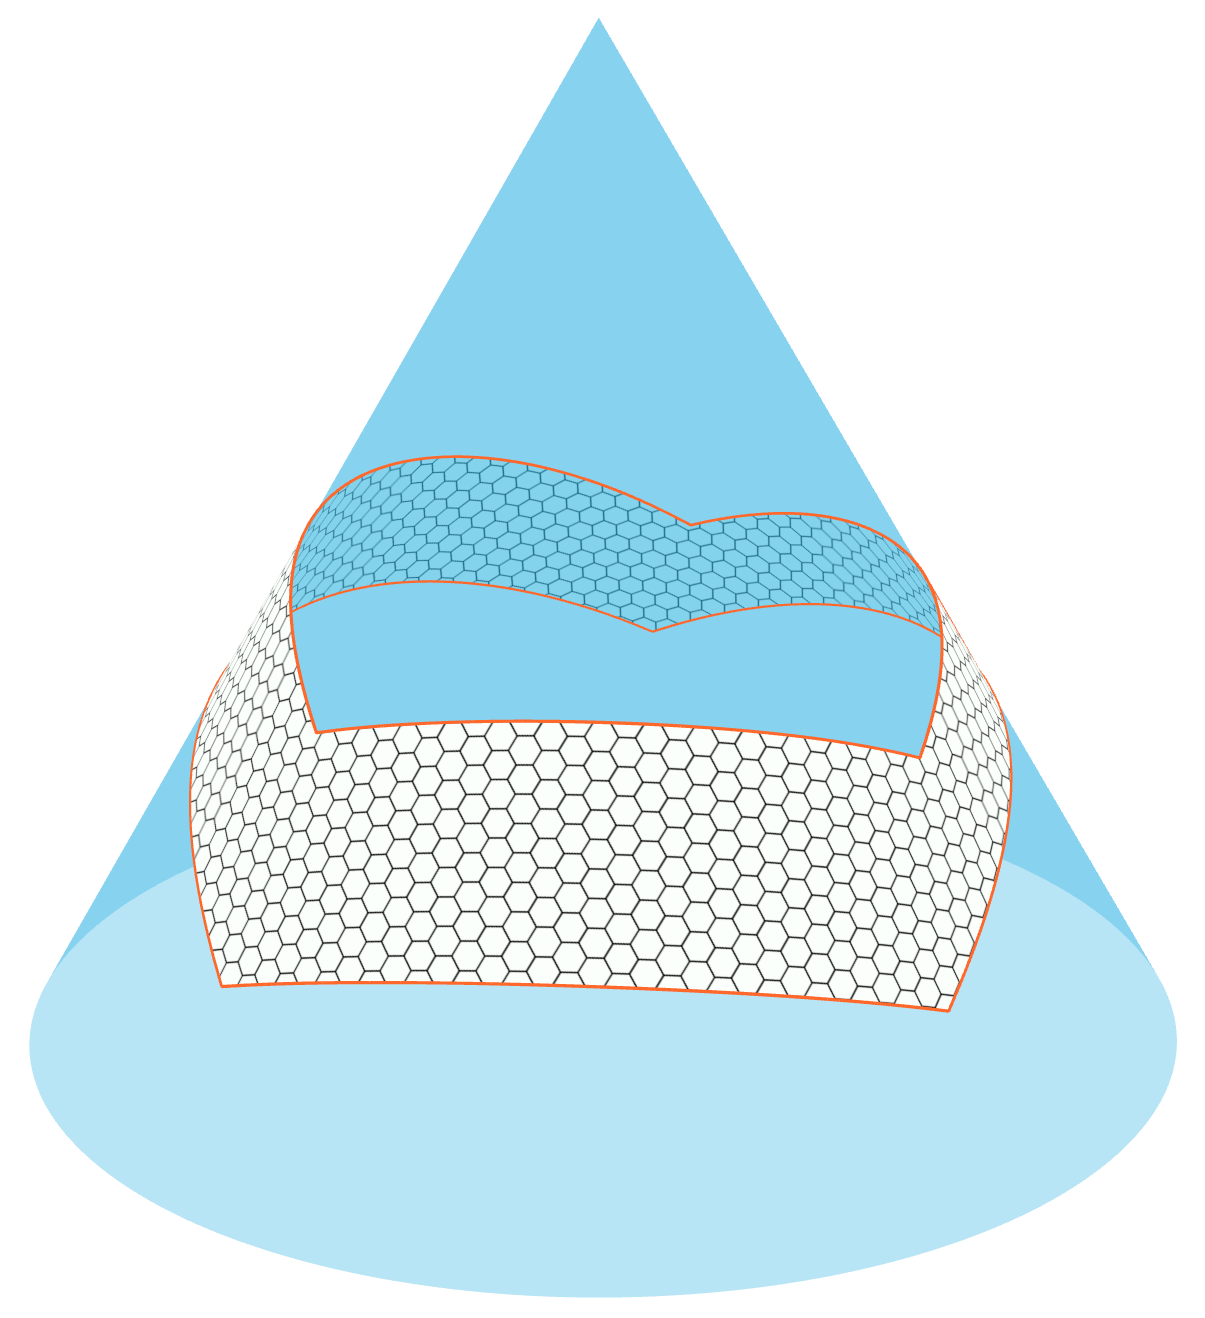
\includegraphics[width=.32\linewidth]{images/conemap_singularities.png}
  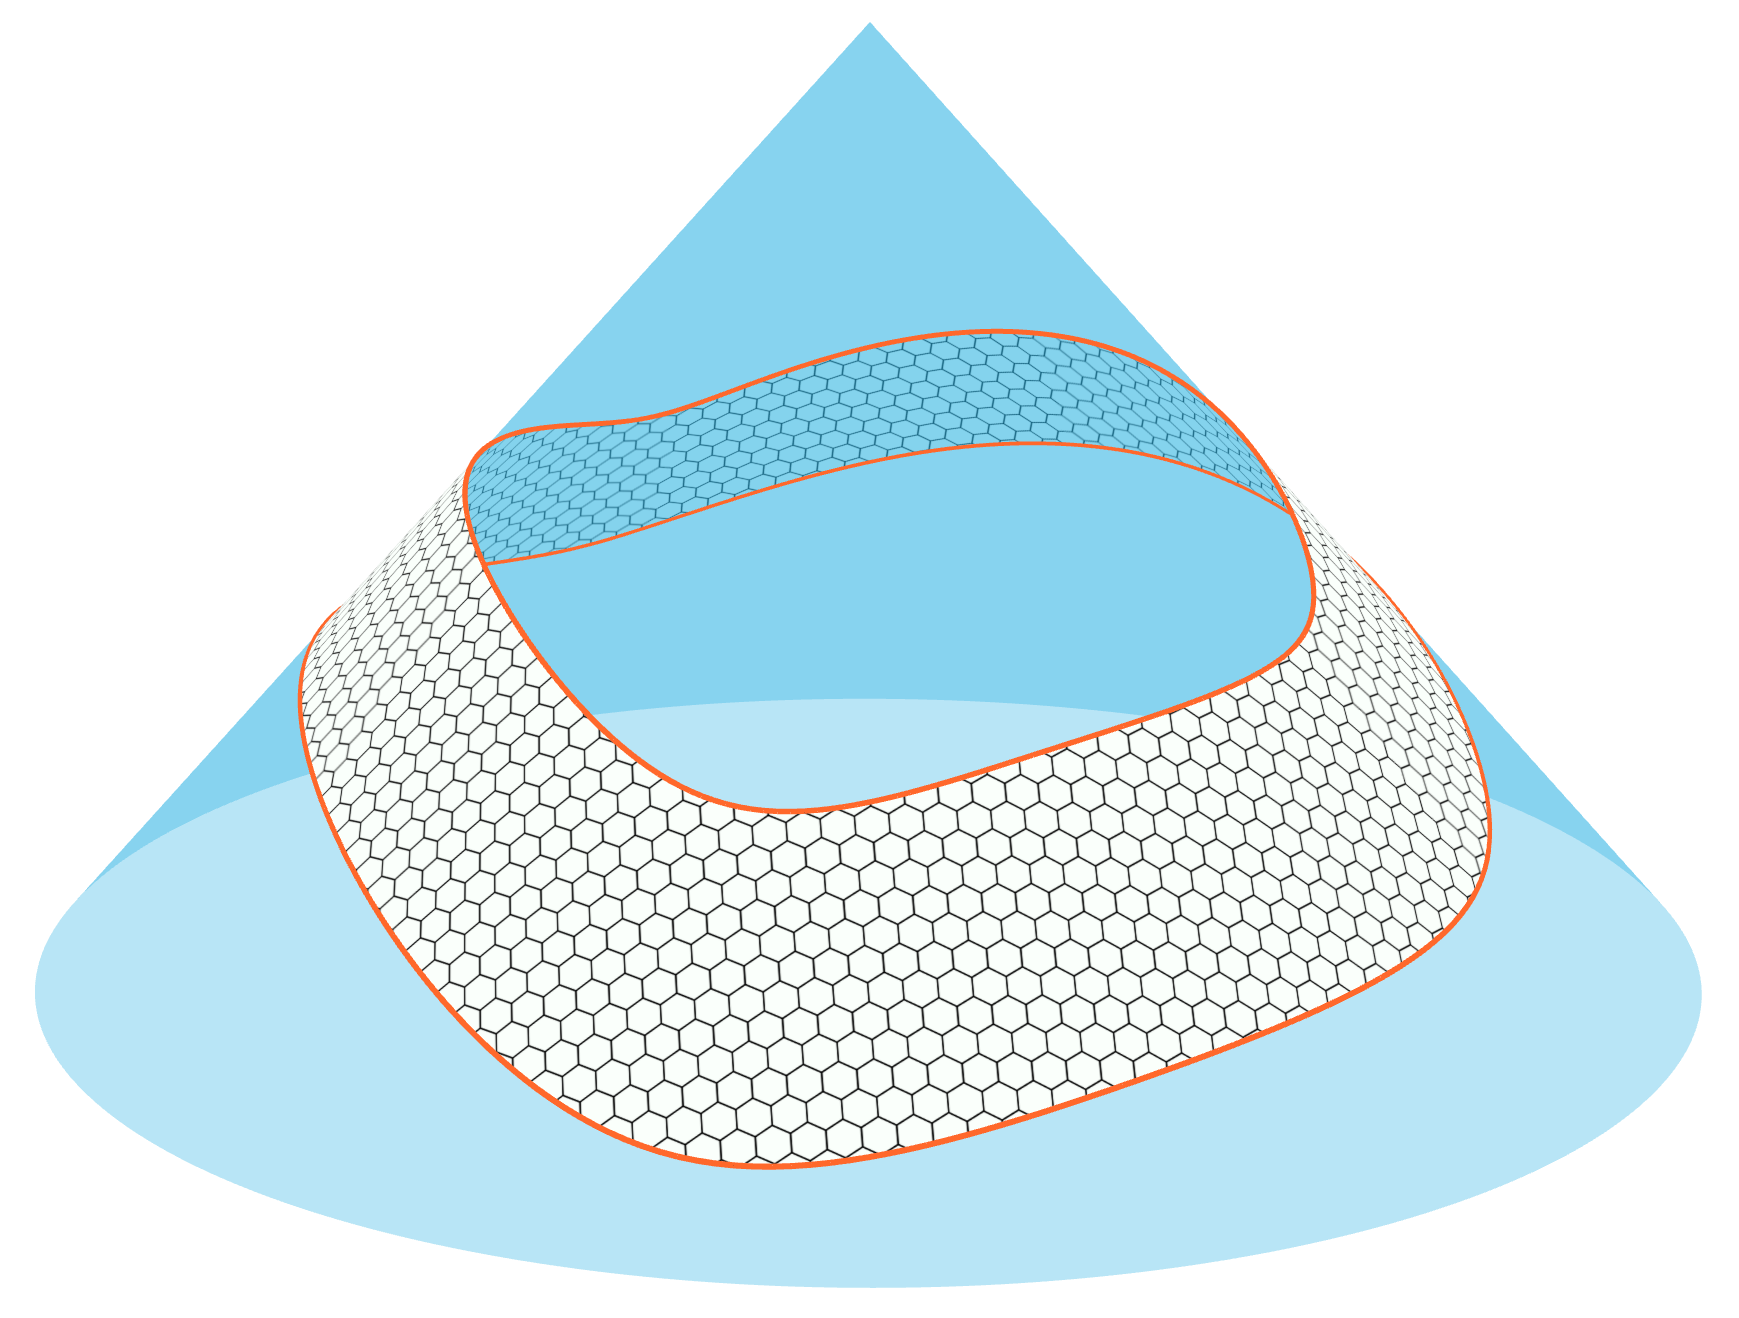
\includegraphics[width=.37\linewidth]{images/conemap_isometric.png}
  \caption{Periodic domains of parameterization of the surfaces shown
    in Figure~\ref{fig:hex_example}.  Left: Map to a cylinder with
    geodesic boundary curves. Middle: Map to a cone of revolution with
    hex-pattern-adapted angle. The domain is a polygon with quantized
    angles. Right: Isometric boundary on a cone with
    hex-pattern-adapted angle.  Panelizations created with the help of
    these maps are shown in Figure~\ref{fig:hex_example}.}
  \label{fig:cone_maps_teaser}
\end{figure}

In this section we describe our algorithm for the creation of periodic
conformal maps for cylindrical meshes/surfaces, i.e., surfaces with
the same topology as a cylinder. First we will review the discrete
conformal maps of~\cite{SSP08}. Then we show how it can be generalized
to yield periodic maps to cylinders or cones.

A smooth \emph{conformal map} between two surfaces is a map that
preserves angles. Intuitively, one can think of a conformal map as a
map that preserves the shape but not the scale of small figures. For
conformal surface parameterization, one looks for conformal
maps from the plane to a surface and vice-versa. These can be used to 
map different patterns onto surfaces in a way that only isotropic
stretch/uniform scaling is applied to the pattern elements.
%
The method described in~\cite{SSP08} is a triangle mesh based
discretization of conformal maps. For each vertex~$v$ of
the surface -- interior or boundary -- we may prescribe an
angle~$\theta_v$ that corresponds to the angle sum of adjacent
triangles in the target mesh.  Starting from an input mesh and target
angles~$\theta_v$, the method calculates new edge lengths for the
triangles of the target mesh such that the angle sums at the target
vertices are as prescribed. This goal is achieved by minimizing a
convex functional.  
%
The prescribed angles have to satisfy a Gauss-Bonnet type condition,
i.e., the angles at interior vertices have to match the angles at the
boundary vertices.  We will state the condition for the special cases
treated later in the article, see Equation~\eqref{eq:theta}.

For the parameterization problem, we want to construct a map from a
surface to the plane. To get a planar target mesh, the target angles
have to be set to~$2\pi$ for all interior vertices, i.e., the angles
of the triangles adjacent to every interior vertex sum up
to~$2\pi$. Thus the computed target triangles can be laid out in the
plane. At the boundaries there is still a certain degree of freedom,
which allows to map the surface to different shapes, e.g., a rectangle
or a more general polygon with prescribed angles. 
%
An alternative choice of boundary conditions yields a target mesh
whose boundary edges have the same lengths as the original mesh. Then
the control over the boundary angles is no longer possible.

This method for the parameterization of triangle meshes can be generalized
to triangle meshes with cylinder topology, see Figure~\ref{fig:discrete_map}. 
Instead of constructing a discrete conformal map from the
surface to the plane, we construct a map to a cylinder or cone, whose image
is isometric to a polygonal region in the plane, see Figure~\ref{fig:cone_maps_teaser}. 
This works with an approach very similar to the previous one. We start 
with the definition of a periodic parameterization.

\begin{definition}
  Let~$M=(V,E,F)$ be a mesh with cylinder topology and vertices~$V$,
  edges~$E$, and triangles~$F$. Let~$D\subset C$ be a region on a
  cone/cylinder of revolution.  A continuous bijection $\Phi:D\to M$
  is called a \emph{discrete periodic parameterization}. $D$ is called
  the \emph{domain of parameterization}.
\end{definition}

In the latter we always assume that the preimages of edges of $M$ are geodesic 
arcs on the cone/cylinder $C$.
For panelization of periodic surfaces we need to make sure, that
different patterns match around the cone or cylinder. This yields
certain restrictions on the cone that serves as domain of parameterization.

\noindent
\begin{minipage}{0.6\linewidth}
  \begin{definition}
    Let~$C$ be a cone with aperture~$\varphi$ and~$\Phi:C\supset D\to M$ be a
    discrete periodic parameterization of a triangle mesh~$M$ with domain~$D$. 
    The map $\Phi$ is called \emph{triangle adapted} if the cone angle $\alpha$ is 
    a multiple of $\frac{\pi}{3}$ and \emph{quad-pattern adapted} if it is a
    multiple of $\frac{\pi}{2}$.
  \end{definition}
\end{minipage}
\begin{minipage}{0.4\linewidth}
  \centering
  \begin{overpic}[height=4cm]{images/cone_angle.pdf}
    \put(38,78){\footnotesize$\varphi$}
    \put(50,60){\footnotesize$1$}
    \put(37,33){\footnotesize$\sin(\varphi/2)$}
    \put(10,10){\footnotesize$\alpha = 2 \pi \sin(\varphi/2)$}
  \end{overpic}
\end{minipage}

This definition ensures that either a quad-, triangle-, or hex-pattern 
fits seamlessly onto the surface after parameterization.

%
\subfilebibliography

\end{document}

%%% Local Variables: 
%%% mode: latex
%%% TeX-master: "article"
%%% End: 
